\chapter{Decomoposizione da monolite a micro-servizi(Assignement 5)}
\label{ch:decomposition}

La precedente versione del software era funzionante ma difficile da mantenere ed aggiornare, data la struttura monolitica.
Esisteva un'unico sorgente che conteneva al suo interno logiche di business, nessun tipo di persistenza e la view tutti assieme.

Per poter decomporre questo monolite sono state eseguite le fasi di: 
\begin{itemize}
  \item Identificazione delle operazioni di sistema.
  \item Decomposizione in servizi, in subdomain seguendo DDD.
  \item Identificazione di API di comunicazione tra servizi.
\end{itemize}

\section{Operazioni di sistema}


\subsection{Knowledge crunching session for the exploration of the problem space}
E' stato utilizzato il metodo Event Storming. 
La tecnica consiste nell'individuare degli eventi di dominio e riportarli al passato su un post-it arancione.
Una volta individuati gli eventi, sono stati scritti su post-it blu i comandi che l'utente svolge per creare l'evento.
In giallo è stato specificato l'attore, la persona che esegue il comando, mentre in verde la view, l'interfaccia software
 con la quale l'utente interagisce.
 Infine, con delle label si sono aggregati i post-it in unità di dominio.
 Si riporta di seguito lo screen della lavagna con i post-it e la relativa legenda.
 \begin{figure}[h!]
    \centering 
    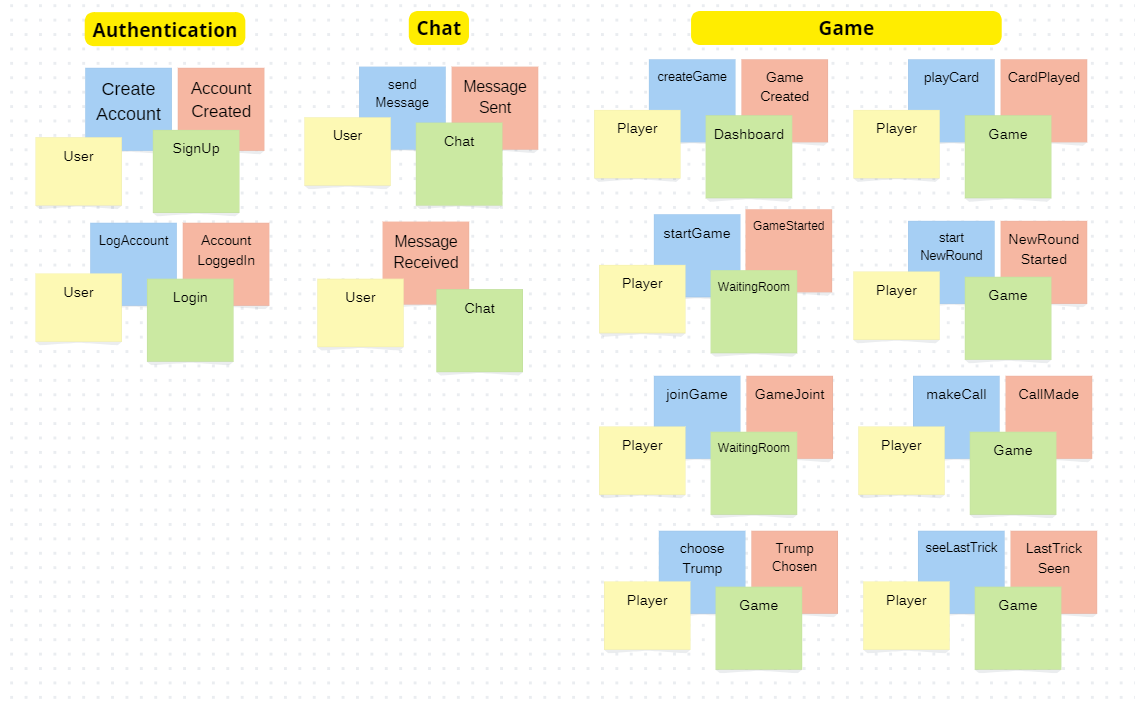
\includegraphics[scale=0.45]{report/img/EventStorming.png}\\[8.5cm]
    \caption{Event Storming}
    \label{event_storming}
\end{figure}

\begin{figure}[h!]
    \centering 
    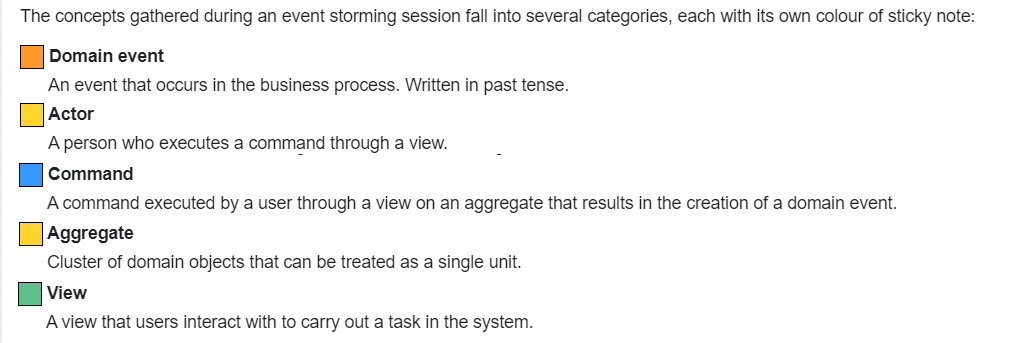
\includegraphics[scale=0.60]{report/img/event_storming_legend.png}
    \caption{Event Storming Legend}
    \label{legend}
\end{figure}


\begin{enumerate}
    \item Account
        \begin{enumerate}
            \item Login
            \item Registrazione
            \item Recupero password
            \item Visualizzazione profilo
            \item Modifica password
            \item Possibilità di scegliere se giocare come ospite o effettuare il login
        \end{enumerate}
    \item Realizzazione partita
        \begin{enumerate}
            \item Creazione partita
            \item Partecipazione partita
            \item gioca carta
            \item Inizio partita
            \item Fine mano
            \item Fine partita
        \end{enumerate}
    \item Chat di gioco
        \begin{enumerate}
            \item chat globale
            \item chat partita
        \end{enumerate}
    \item Possibilità di scegliere un compagno di squadra
    \item Scelta del seme, parole consentite
    \item Modalità di gioco 11 a 0
    \item Gestione punteggio
        \begin{enumerate}
            \item Calcolo totale e parziale (Gestione per ogni mano) del punteggio
            \item Maraffa/Cricca (+3 punti)
        \end{enumerate}
    \item Servizio gestione utenti
    \item Salvataggio statistiche
    \item Realizzazione GUI
        \begin{enumerate}
            \item Refactor della GUI esistente
            \item Rinnovamento GUI
        \end{enumerate}
\end{enumerate}

\subsection{Casi d'uso}
Si riporta di seguito lo schema dei casi d'uso che modella l'interazione dell'utente con l'applicazione.
\begin{figure}[h!]
\centering 
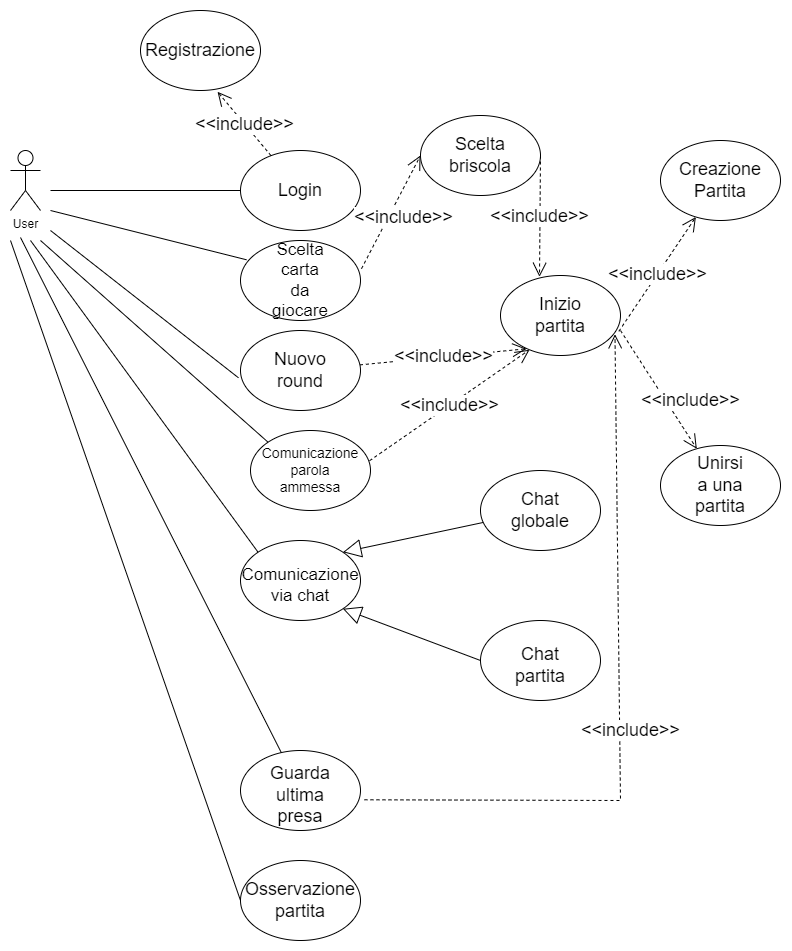
\includegraphics[scale=0.45]{report/img/Casi_duso.png}
\caption{Schema dei casi d'uso}
\label{use_case}
\end{figure}

\newpage 

\section{Decomposizione in servizi}


\subsection{Bounded Context}
Analizzando il dominio di MaraffaOnline, sono stati identificati i tre principali bounded context che andranno poi a definire (ad alto livello) i servizi e alcune delle loro API all'interno dell'architettura.
Nella figura si può osservare un primo bounded context, colorato di azzurro, che modella l'autenticazione dell'utente:
    \begin{itemize}
        \item \textbf{User:} persona che possiede l'account
        \item \textbf{Statistic:} dati dell'utente relativi al gioco come numero di vittorie, sconfitte, partite giocate e maraffe
        \item \textbf{Authentication:} accesso all'applicativo MaraffaOnline da parte dell'utente
    \end{itemize}
Il secondo bounded context, colorato di verde, modella la partita:
    \begin{itemize}
        \item \textbf{Game:} partita
        \item \textbf{Team:} squadra composta da numero di giocatori / 2
        \item \textbf{Score:} punteggio delle due squadre
        \item \textbf{Statistic:} dati relativi ai game giocati
        \item \textbf{Trick:} presa di quattro carte da parte di un giocatore
        \item \textbf{Round:} 10 prese
        \item \textbf{Card:} carta
        \item \textbf{Player:} giocatore
        \item \textbf{Deck:} mazzo
        \item \textbf{Hand:} carte che ha in mano un giocatore
    \end{itemize}
Infine l'ultimo, di colore arancione, modella la chat:
    \begin{itemize}
        \item \textbf{Chat:} chat di gioco
        \item \textbf{Message:} messaggio inviato nella chat
        \item \textbf{User:} persona che invia il messaggio
    \end{itemize}
È importante notare che il concetto di user/player è polisemico: vi sono tre rappresentazioni diverse per afferire allo stesso concetto.
\begin{figure}[h!]
    \centering 
    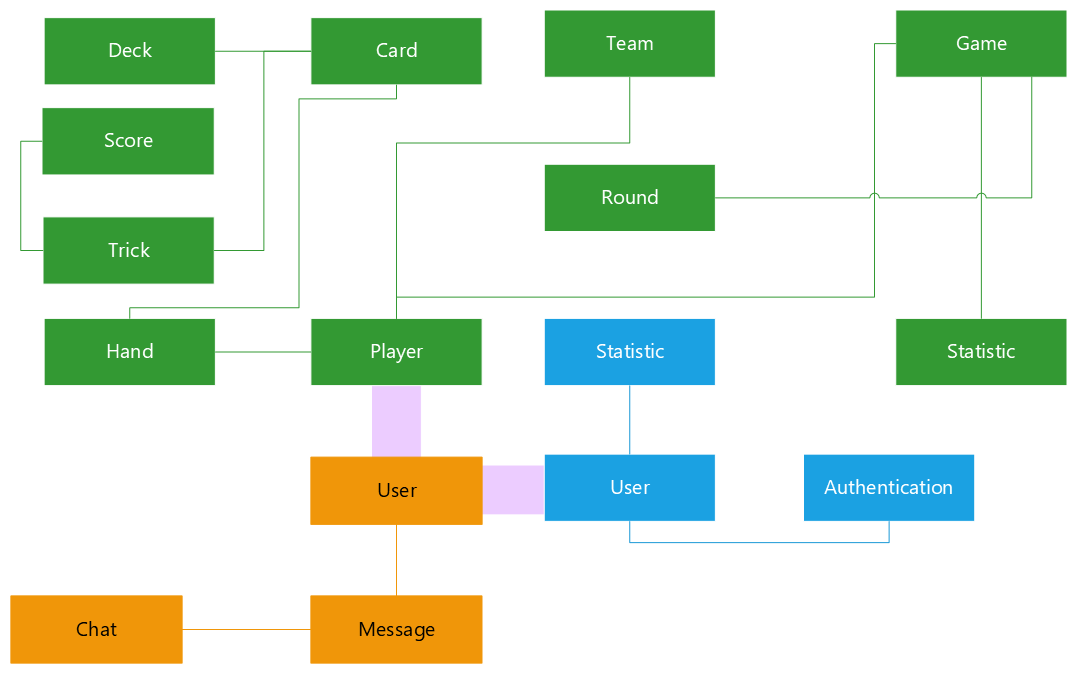
\includegraphics[scale=0.75]{report/img/BoundedCTX.png}
    \caption{Context Map}
    \label{bounded_context}
\end{figure}
\newpage


\subsection{Schema architettura}

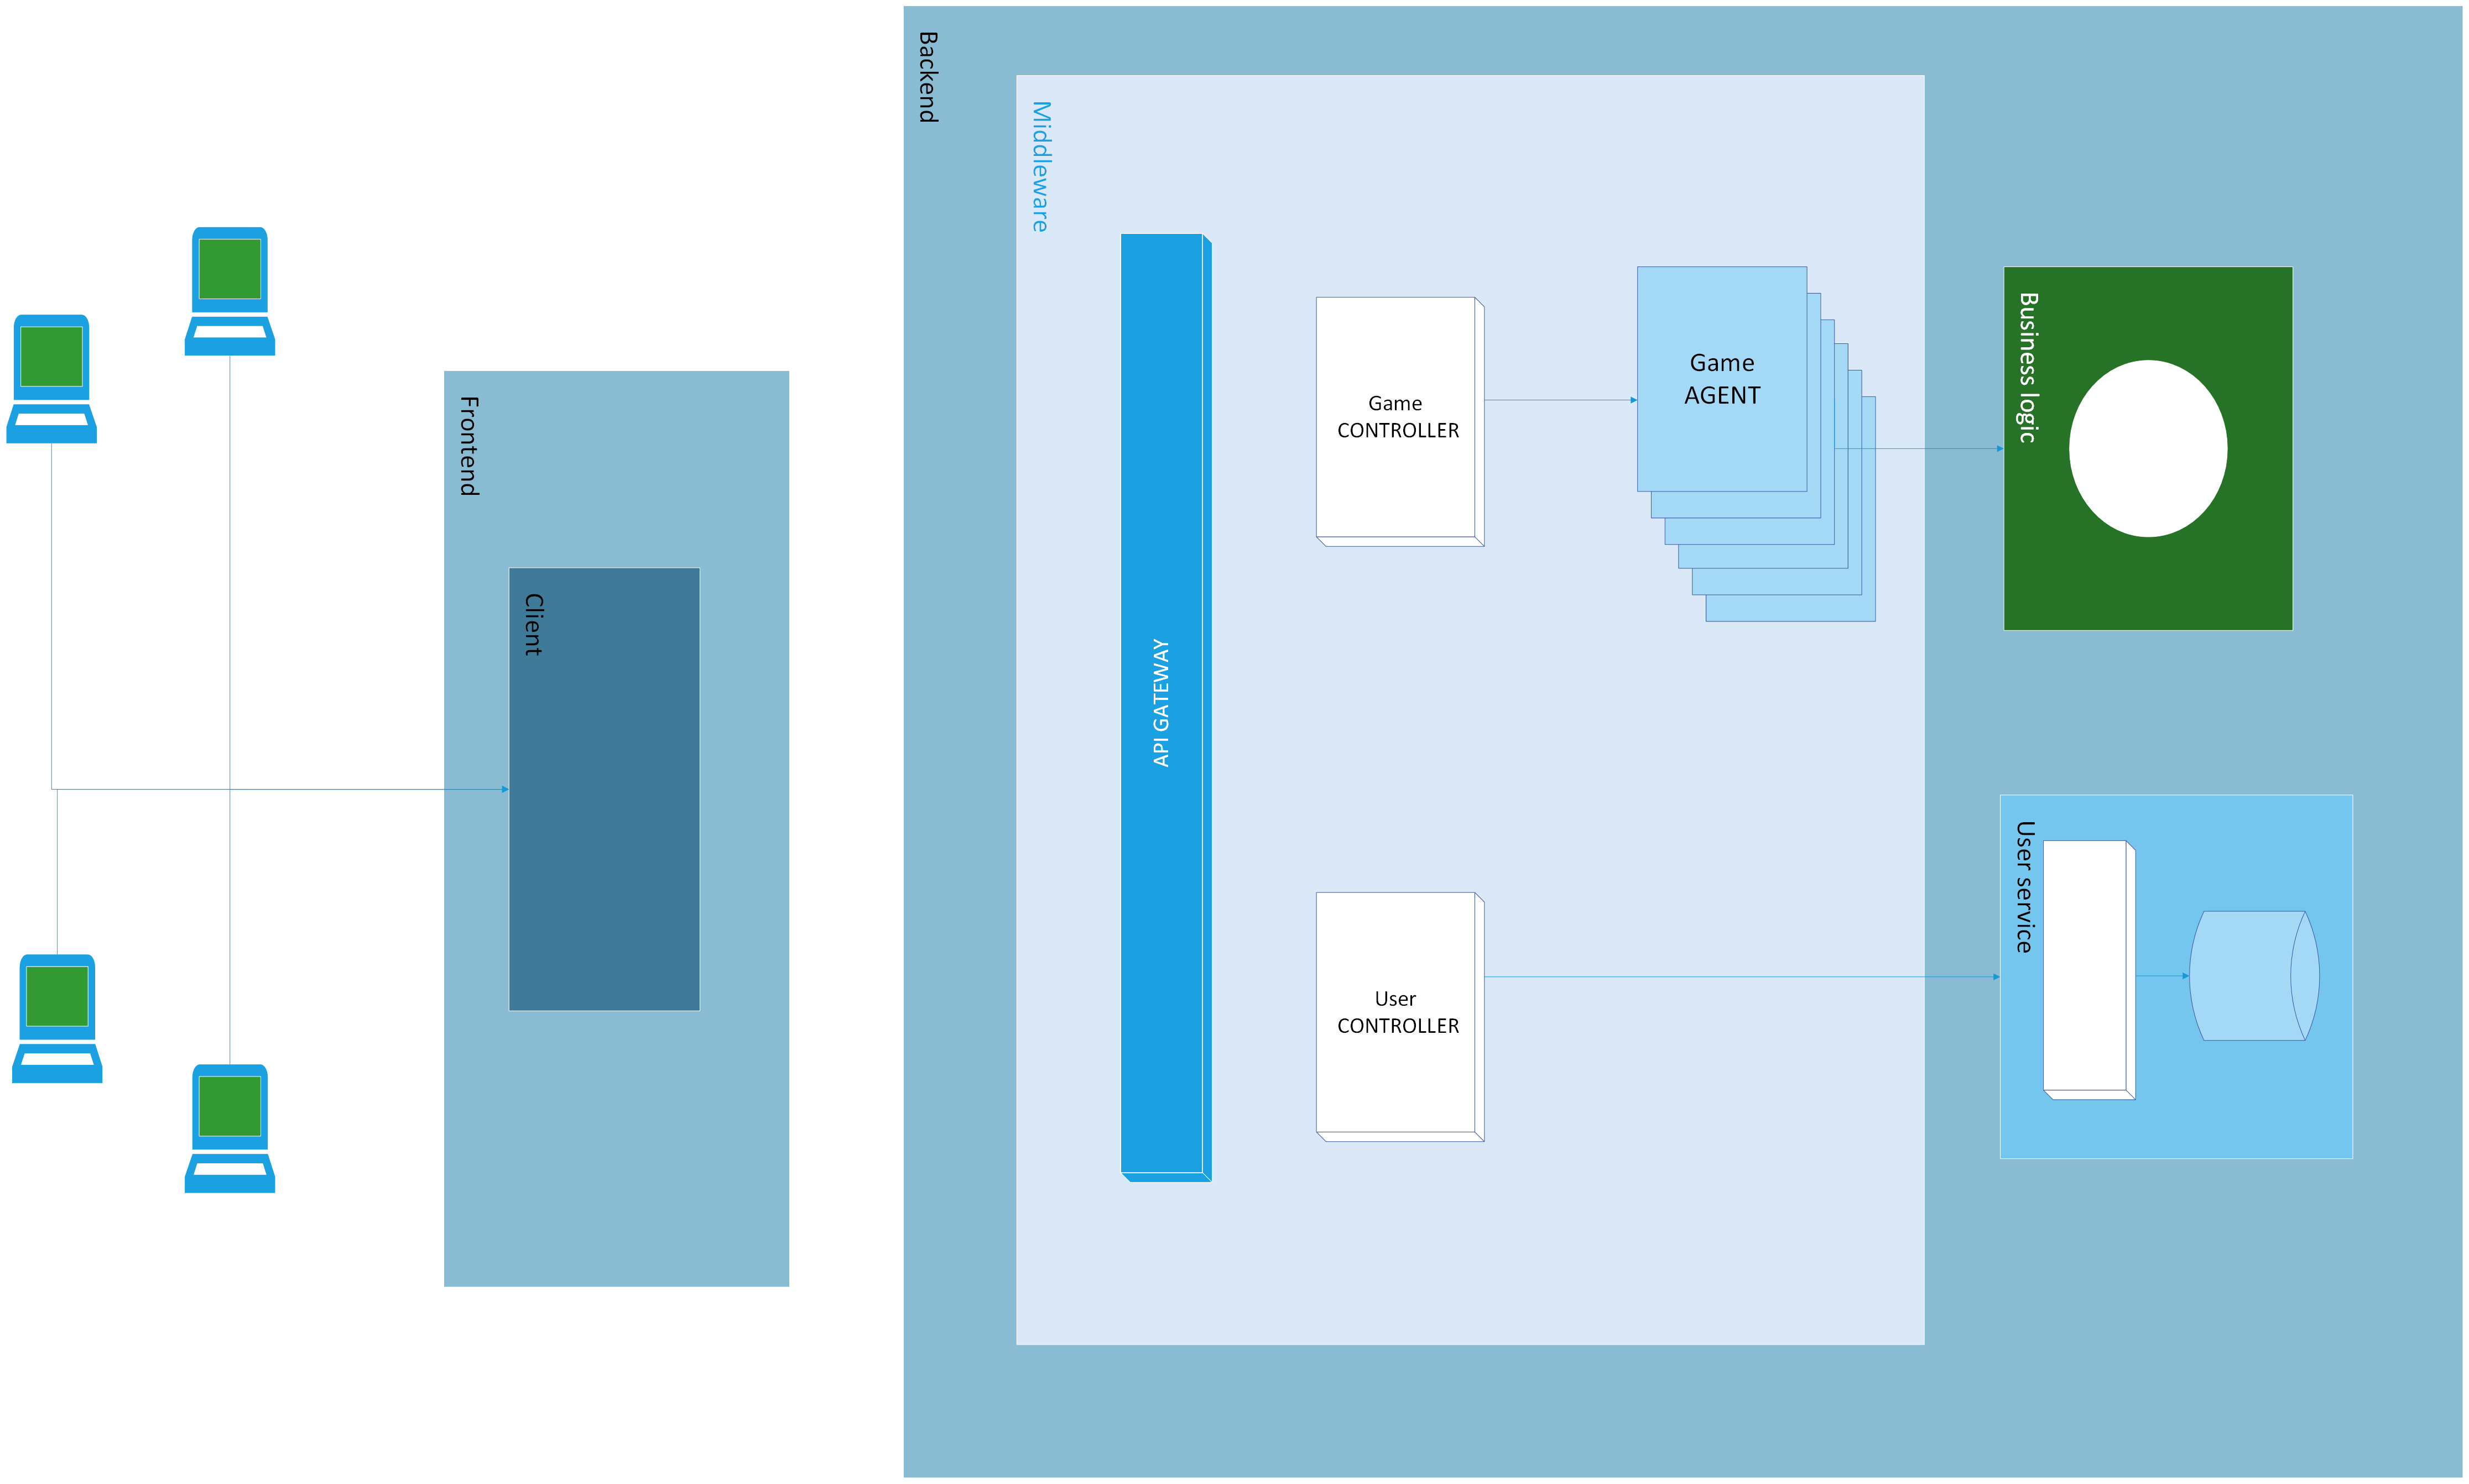
\includegraphics[width=16cm]{report/img/Architecture.png}\\[8.5cm]


\newpage
\section{Comunicazione tra servizi}


\subsection{API gateway}
Sono state implementate diverse forme di comunicazione tra servizi in base alle caratteristiche del messaggio che viene scambiato. Si è scelto di utilizzare la comunicazione REST nella maggior parte dei servizi, visto la sua interoperabilità.
Non è stato necessario implementare un vero e proprio broker di messaggi, ma è stato implementato un servizio denominato middleware che svolge il ruolo di API gatetway delle richieste dai client verso il sistema.

Queste chiamate non sono obbligatoriamente dirette verso il servizio interessato, ma possono anche essere routine che effettuano molteplici chiamate per ottenere il risultato desiderato. 
Implementare queste chiamate direttamente nel front-end avrebbe reso il codice molto più complesso e difficile da mantenere, e la gestione di partite multiple sarebbe stata molto più complicata.

\vspace{1cm}

Non è stato implementato nessun meccanismo di discovery per scoprire l'indirizzo degli altri servizi, è stato sfruatta la tecnologia built-in di docker che permette di poter utilizzare degli alias e nascondere al proprio interno i meccaniscmi di registration, questo comunque implica che tutto debba essere sempre mantenuto nell'ambiene virtualizzato e quindi ogni  futueo servizio containerizzato.

\vspace{1cm}

Si è seguito un approccio modulare nello sviluppo di questo componente che, in un primo step, conteneva soltanto la logica di gestione delle partite, al quale sono stati aggiunti i moduli per la comunicazione con il servizio degli utenti e della business logic. Ogni modulo segue la stessa struttura, ossia una classe denominata controller che si occupa esclusivamente della dichiarazione delle rotte HTTP e che a sua volta contiene un service. Ogni servizio contiene poi le logiche di calcolo e crea un JSON di risposta che viene passato al controller che lo invia come risposta HTTP, questo per poter separare completamente e rispettare il principio di single responsibility.

Nel modulo contenente le logiche di gioco è stato necessario aggiungere un ulteriore strato di separazione alla struttura controller-service, data la struttura multi-attore della gestione delle partite che non permetteva una separazione netta. Quindi è stato aggiunto, tra il controller e il service, un componente ibrido per poter comunque avere servizi indipendenti.

Questa separazione, oltre a essere una buona pratica, è stata scelta per poter effettuare del testing comodamente soltanto sui servizi, testando quindi solamente la parte relativa all'elaborazione di una risposta.

\subsection{Websocket module}

L'interazione con il frontend avviene prevalentemente tramite il protocollo HTTP, ma per la gestione di alcuni aspetti in tempo reale sono state introdotte le WebSocket.
Questo componente è stato creato, ad esempio, per la gestione delle chat di gioco, in modo che i giocatori possano comunicare tra loro in tempo reale. Ogni client, istanziato sul computer degli utenti, effettua una connessione WebSocket con il middleware utilizzando come endpoint il proprio UUID, che viene assegnato automaticamente all'avvio, e lo username del giocatore, dopo aver effettuato il login. Il middleware contiene al proprio interno una mappa di tutti i client e giocatori connessi con la relativa WebSocket e una classe che espone due metodi per inviare messaggi a un singolo giocatore o effettuare un messaggio broadcast a tutti i giocatori connessi.

Il modulo di game si occupa di gestire le partite, quindi è l'unico che può sapere quali giocatori devono ricevere determinati messaggi relativi a una singola partita. Per utilizzare il servizio di WebSocket, è stata implementata una semplice interfaccia all'interno dell'attore di gioco con la quale si effettuano chiamate "onEvent". Ogni volta che un particolare evento si verifica, un'invocazione a queste chiamate permette di inviare messaggi alle WebSocket dei giocatori interessati.

